% !TeX spellcheck = de_DE
\chapter{Friedmann-Gleichung\label{chapter:thema}}
\lhead{Friedmann-Gleichung}
\begin{refsection}
\chapterauthor{Andri Hartmann und Tobias Schuler}
\printbibliography[heading=subbibliography]
%\epstopdfsetup{outdir=./} %Sonst koennen keine Grafiken von eps-to-pdf konvertiert werden
\lhead{Einleitung zur Friedmann-Gleichung}
\rhead{}
\begin{quote}
	\textit{Wir dürfen das Weltall nicht einengen, um es den Grenzen unseres Vorstellungsvermögens anzupassen, wie der Mensch es bisher zu tun pflegte. Wir müssen vielmehr unser Wissen ausdehnen, sodass es das Bild des Weltalls zu fassen vermag.}\footnote{Sir Francis von Verulam Bacon (1561 - 1626)}
\end{quote}
In diesem Kapitel möchten wir euch helfen, gemäss dem oben erwähnten Zitat, das Bild des Weltalls fassen zu vermögen. Um dies zu tun, werden wir versuchen, das Gebilde, welches wir Universum nennen, unter Zuhilfenahme der physikalischen Gesetze in einen mathematischen Kontext zu bringen.

\section{Vorgeschichte}
Mit der Formulierung der Allgemeinen Relativitätstheorie durch Albert Einstein war es erstmals möglich,
sich seriös Gedanken über die Geschichte des
Universums zu machen. An dieses Problem haben sich anfangs der 20er Jahre bekannte Wissenschaftler wie Einstein, deSitter, Friedmann und Lemaitre gemacht. 
Zu dieser Zeit gab es wenig bis keine experimentellen Daten, die Aussagen über Geometrie oder Dynamik des Weltalls hätten treffen können. So kam es, das unter den führenden Astronomen das Bild eines statischen Universums grosse Empathie erhielt.

Durch die Entdeckung der Fluchtbewegungen von Galaxien mithilfe der kosmologischen Rotverschiebungen gelang es 1929 dem US-amerikanischen Astronomen Edwin Hubble, die damalige Vorstellung eines statischen Kosmos zu widerlegen. Diese Entdeckung hatte zur Folge, dass man jetzt ein Modell mit einem sich veränderndem Weltradius brauchte.
\pagebreak
\section{Skalenfaktor a\label{Section:Skalenfaktor}}
Um ein dynamisches Universum beschreiben zu können, führen wir ein dreidimensionales Koordinatensystem ein, welches sich mit der relativen Bewegung von Galaxien mitbewegen kann. In einem solchen System besitzen die Objekte fixe Koordinaten und sind somit wie in einem Raster eingefroren. Die Einheit des Rasters wird durch den {\em Skalenfaktor} $a$ ausgedrückt und ist eine Funktion der Zeit. Ein zweidimensionales Raster ist in Abbildung \ref{friedmann:friedmannRaster} zu sehen. Die drei Kreise stellen Galaxien dar. Die Linie zwischen der roten und blauen Galaxie zeigt den Abstand. Dehnt sich nun das Universum aus, dehnt sich das Raster mit, wie auf dem zweiten Plot zu sehen ist. Die Grösse der Galaxien und die Position auf dem Raster bleiben gleich, der Abstand zwischen den Galaxien hat sich aber verändert. 

%\begin{figure}[h]
%	\centering
%	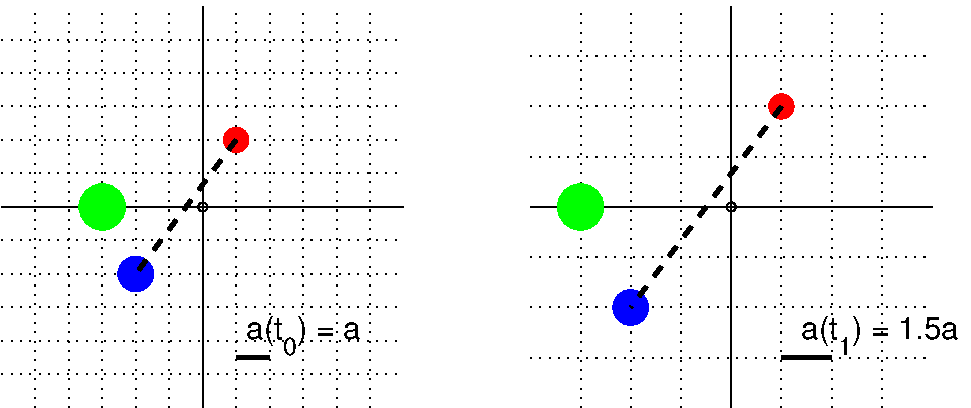
\includegraphics[width  = \textwidth]{friedmann/images/rasterFriedmann}
%	\caption{Raster ums Universum für zwei verschiedene Skalenfaktoren}
%	\label{friedmann:friedmannRaster}
%\end{figure}%

\subsection{Mathematische Beziehungen im Koordinatensystem \label{friedmann:Beziehungen im Koordinatensystem}}
Die Distanz zwischen zwei Punkten A und B entspricht 
\begin{equation}
D_{AB}(t)\, = \sqrt{a^2(t)\Delta_{AB}\,x^2 + a^2(t)\Delta_{AB}\,y^2 + a^2(t)\Delta_{AB}\,z^2}\, =\, a(t) \sqrt{\Delta_{AB}\,x^2 + \Delta_{AB}\,y^2 + \Delta_{AB}\,z^2}
\end{equation}
F\"{u}r die Geschwindigkeit, mit der sich die beiden Punkte relativ zueinander bewegen, gilt 
\begin{equation}
\varv_{AB}(t) = \dfrac{dD_{ab}}{dt} 
= \dot{a}(t) \sqrt{\Delta_{AB}\,x^2 + \Delta_{AB}\,y^2 + \Delta_{AB}\,z^2}
\end{equation}
Um nun Aussagen über die Dynamik des Universums zu machen, die nicht von der fiktiven Wahl des Skalenfaktors abhängen, teilen wir die Geschwindigkeit durch den Skalenfaktor $a$.
\begin{equation}
\frac{\varv_{AB} }{D_{AB}} = \frac{\dot{a}}{a}
\label{friedmann:geschwindigkeit}
\end{equation}
%\begin{satz} [Hubble-Konstante]
%	Die Ableitung des Skalenfaktors dividiert durch den Skalenfaktor entspricht der Hubble-Konstante.
%	\[
%	\frac{\dot{a}}{a} = H
%	\]
%\end{satz}
\begin{satz}[Kosmologisches Prinzip]
\label{Prinzip:kosmologisches Prinzip}
Das kosmologische Prinzip besagt, dass auf einer grossen Längenskala kein Ort im Universum gegenüber einem anderen ausgezeichnet ist. Diese Annahme bedingt zwei Eigenschaften, Isotropie und Homogenität.\\
Isotropie  bezeichnet die Unabhängigkeit einer Eigenschaft von der Richtung.
Homogenität bezeichnet die Gleichheit einer physikalischen Eigenschaft über die gesamte Ausdehnung eines Systems.
\end{satz}
Gemäss Satz (\ref{Prinzip:kosmologisches Prinzip}) und der Eigenschaft unseres Koordinatensystems, Kap.(\ref{Section:Skalenfaktor}), bleibt die Masse in einem Einheitskubik konstant über die Zeit. Somit ist die Masse $M$ in einem Würfel mit Dimension $\Delta x$, $\Delta y$ und $\Delta z$ 
\begin{equation}
M_{xyz} = \nu \, \Delta x \, \Delta y \, \Delta z
\end{equation}
Der Parameter $\nu$ beschreibt die Massendichte in einem Einheitsquader und ist somit von der Wahl von $a$ abhängig, jedoch konstant über die Zeit. Das Volumen des Würfels ist bekanntlich 
\begin{equation}
V_{xyz} = a^3 \Delta x \Delta y \Delta z
\end{equation}
und folglich kann die Massendichte geschrieben werden als
\begin{equation}
\rho = \frac{M_{xyz}}{V_{xyz}} = \frac{\nu}{a^3}
\label{friedmann:dichte}
\end{equation}

Es stellt sich nun die spannende Frage: Wie ändert sich der Skalenfaktor mit der Zeit? Und eben diese Frage wird mit der Friedmann-Lema\^{i}tre Differentialgleichung beantwortet.


%\section{Expansion des Universums}
%Albert Einstein schlug 1917 mit dem Formalismus der ART ein statisches Universum vor. Damit sein sphärisches Universum($\kappa = +1$) einen konstanten Weltradius hatte, Einstein empfand das als am ästhetischsten,  führte er den $\Lambda$-Term ein. Im gleichen Jahr fand Willem de Sitter ein flaches Universum($\kappa = 0$), das dynamisch aber materiefrei war. Damit verstösst es gegen das Machsche Prinzip.\footnote{Das Machsche Prinzip sagt unter anderem aus, dass es ohne Materie keine Geometrie geben kann.} Alexander Friedmann leitete 1922 eine Gleichung her, die sämtliche Universen enthält, auch den statischen Einstein-Kosmos. Mit seiner Gleichung konnte er dynamische, ja sogar pulsierende Universen beschreiben. Zu dieser Zeit fand die Vorstellung eines dynamischen Universums aber von den meisten Wissenschaftlern, allen voran von Albert Einstein, keine Akzeptanz. Erst mit der Entdeckung der Rotverschiebung durch Hubble und der Lösung eines expandierenden Universum von Lema\^{i}tre, der auf dem gleichen Gebiet wie Friedmann arbeitete, verschafften sich die Friedmann-Lema\^{i}tre-Weltmodelle verdienten Zulauf.
 
\section{Alexander Friedmann und Georges Lema\^{i}tre}
Die sogenannte Friedmann-Lema\^{i}tre-Gleichung beschreibt das Verhalten des Universums nach der Inflation des Kosmos im Rahmen des Standard-Urknall-Modells. Die {\em Energiedichte} $\rho$, die {\em Krümmung} $\kappa$ und die {\em kosmologische Konstante} $\Lambda$ sind die Parameter der Gleichung.
\begin{equation}
\left(\frac{\dot{a}}{a}\right) ^2 = \frac{8 \pi G}{3} \rho - \frac{\kappa c^2}{a^2} + \frac{\Lambda c^2}{3}
\end{equation}

%\subsection*{Lösungen der Gleichung für verschiedene Parameter}
Bevor wir beginnen, die Gleichung herzuleiten, können wir schon jetzt verschiedene Lösungen für unterschiedliche Parameterwerte diskutieren. Das hilft uns später beim Rekonstruieren der Geschichte des Universums.

\subsection{Masseloses Universum}
%Sie könnten zum Beispiel könnten zum Beispiel mit einem leeren Universum beginnen (rho = 0), und die Gleichung einfach mal für den zweiten und dritten Term lösen. Rein mathematisch, ohne die Physik schon zu untersuchen. Hier können Sie den Trick mit der zusätzlichen Ableitung?? erklären. Damit zeigen Sie schon mal, dass die Gleichung eine Vielzahl spannender Lösungen hat.
Setzen wir $\rho = 0$, entspricht dies einem masselosen Universum.  Wir schreiben die Gleichung ohne den ersten Term
\[\left(\frac{\dot{a}}{a}\right) ^2 = - \frac{\kappa c^2}{a^2} + \frac{\Lambda c^2}{3}\]
Nun sind noch zwei Terme übrig. Separiert man sie, findet man eine Lösung wie folgt
\begin{enumerate}
	\item $\kappa = 0$ 
		\begin{align*}
			\left(\frac{\dot{a}}{a}\right) ^2 &= \frac{\Lambda c^2}{3}  &&| \cdot a^2 \\
			\dot{a} ^2 &= \frac{\Lambda c^2 a^2}{3}  &&|\sqrt{...}\\
			\dot{a} &= \sqrt{\frac{\Lambda c^2}{3}} a &&|\sqrt{\frac{\Lambda c^2}{3}} := E \ge 0 \, (!)\\
			\dot{a} &= E \cdot a &&|\int ...\, dt \\
		\end{align*}
		
	\begin{equation}\label{friedmann:Lambda}
		\boxed{a = e^{E \cdot t}}
	\end{equation}
	
		 
Mit $\kappa = 0$ gibt es zwei mögliche Ausprägungen für das Universum, entweder ist $E = 0$ oder $E > 0$. Im ersten Fall wäre das Universum statisch und wäre für alle Zeit gerade so gross wie der Skalenfaktor. Im zweiten Fall würde sich das Universum exponentiell ausdehnen.
		
	\item $\Lambda = 0$ 
		\begin{align*}
			\left(\frac{\dot{a}}{a}\right) ^2 &= - \frac{\kappa c^2}{a^2}  \qquad &&| \cdot a^2\\
			\dot{a} ^2 &= - \kappa \, c^2 \qquad &&|\sqrt{...}\\
			\dot{a} &= \sqrt{- \kappa}\, c \qquad &&|\int ...\, dt\\
		\end{align*}
		\begin{equation}	\label{friedmann:Kappa}
			\boxed{a = \sqrt{- \kappa}\, c \cdot t}
		\end{equation} 
		
Auch hier gibt es zwei mögliche Ausprägungen. Wie vorhin könnte $\kappa = 0$ sein, oder $\kappa < 0$. In diesem Fall würde das bedeuten, es entsteht entweder kein Raum, da der Skalenfaktor $a$ nie anwächst, oder aber das Universum wächst linear mit der Zeit an.
	
\end{enumerate}

\subsection{Universum mit Masse}
Wie vorhin schon angedeutet, steht $\rho$ für die Massendichte im Universum. Ist das Universum massenlos, ist die Dichte null. Gehen wir aber davon aus, dass im Universum Materie vorhanden ist, findet man eine weitere Lösung der Differentialgleichung. Zu beachten ist, dass die Dichte abhängig von der Ausdehnung ist. Als Gedankenstütze kann man sich eine geschlossene Box gefüllt mit einem homogenen Gas vorstellen. Vergrössert sich die Box nun wie sich das Universum ausdehnt, nimmt die Dichte ab solange kein Gas hinzugefügt wird. Dies ist auch in Abbildung (\ref{friedmann:friedmannRaster}) zu sehen. Das Raster ist im zweiten Plot grösser geworden, die Masse im Raster hat aber nicht zugenommen. Die Ausdehnung geschieht in einem dreidimensionalen System kubisch, die Massendichte muss also kubisch abnehmen. Damit die Gleichung lösbar ist, vernachlässigen wir den $\Lambda$- und $\kappa$-Term. Für die Dichte setzen wir (\ref{friedmann:dichte}) ein. 
\[\left(\frac{\dot{a}}{a}\right) ^2 = \frac{8 \pi G}{3} \frac{\nu}{a^3}\]
Weiter können wir $\nu$ so wählen, dass sich der konstante Term als eins schreiben lässt.

\begin{align*}
\left(\frac{\dot{a}}{a}\right) ^2 = \frac{1}{a^3} \quad &\Leftrightarrow \quad \dot{a}^2 = \frac{1}{a} \\
\frac{da}{dt} = \frac{1}{\sqrt{a}} \quad &\Leftrightarrow \quad
\frac{dt}{da} = \sqrt{a} \\
\int 1 \, dt = \int \sqrt{a}\, da  \quad &\Leftrightarrow \quad
t = \frac{2}{3}\, a{^\frac{3}{2}}
\end{align*}
\begin{equation} \label{friedmann:Masse}
\boxed{a = \frac{3}{2}\, t^{\frac{2}{3}}}
\end{equation}


\subsection*{Diskussion der Lösungen}
Wir finden also für jeden Term in der Gleichung eine andere Beschreibung der Bewegung des Universums. Betrachten wir die Anfangsgleichung genauer, können wir herauslesen, welcher Term bei einer gegebenen Grösse $a$ dominierend war.
\begin{align*}
\left(\frac{\dot{a}}{a}\right) ^2 =\;\frac{8 \pi G}{3} \rho\; &- \;\frac{\kappa c^2}{a^2}\; + \;\frac{\Lambda c^2}{3} \\
\left(\frac{\dot{a}}{a}\right) ^2 = \;\frac{1}{a^3}\; &-\;\frac{\kappa c^2}{a^2}\; +\; \frac{\Lambda c^2}{3}
\end{align*}
Für kleine Werte von $a$ wird der erste Term dominieren, für mittlere Werte von $a$ der Zweite, und für grosse Werte dominiert der letzte Term. Das heisst, die Lösungen setzen sich in zeitlicher Reihenfolge wie folgt zusammen:
Gleichung (\ref{friedmann:Masse})  dominiert zu Beginn, dann mischt sich Gleichung (\ref{friedmann:Kappa}) ins Spiel, und am Schluss dominiert Gleichung (\ref{friedmann:Lambda}) über das Schicksal des Universums.
\subsection{Herleitung der Differential-Gleichung}
Im folgenden Abschnitt versuchen wir die Bedeutung der einzelnen Terme physikalisch zu hinterlegen. Das ist nicht immer ganz einfach, denn die Differential-Gleichung wurde unter anderem mithilfe der Einstein'schen Feldgleichungen hergeleitet worden. In diesem Kapitel werden wir aber nicht so weit gehen, trotzdem können wir einige interessante Relationen mithilfe der klassischen Physik herleiten.
\subsubsection{Newtonscher Ansatz}
Um die relative Beschleunigung zweier Punkte im Universum zu beschreiben, wird von folgendem Ansatz ausgegangen: Ein Beobachter befindet sich im Ursprung des Koordinatensystems und ist in Ruhe. Um nun die Kraft auf einen Körper der \textbf{Masse} $m$ im \textbf{Abstand} $D$ zu berechnen, denkt man sich eine Kugelschale um den Ursprung mit \textbf{Radius} $D$. Die Kraft auf den Körper verhält sich wie die Punktmasse aller  einzelnen Körper in der Kugel im Ursprung gedacht.
Im folgenden Abschnitt werden die in Kap.(\ref{friedmann:Beziehungen im Koordinatensystem}) hergeleiteten Formeln angewendet. Einfachheitshalber schreiben wir für den Abstand im Grid
\[ \sqrt{\Delta x^2 + \Delta y^2 + \Delta z^2} := R \]
und für das Volumen V der Kugel
\[V_\text{Kugel} = \frac{4 \pi }{3} a^3 R^3\]
Gemäss Newton ergibt sich die Gravitationskraft aus
\begin{equation}
F_G = -\frac{m M G}{D^2}
\end{equation}
Da die Gravitationskraft zwecks Vereinfachung des Modells als einzige Kraft eingesehen wird, gilt für die Beschleunigung mit 
\[F = m A\]
\[A = - \frac{M G}{D^2} = \ddot{a} R \quad\Leftrightarrow\quad \ddot{a} = \frac{- M G}{a^2 R^3} \quad\Leftrightarrow\quad \frac{\ddot{a}}{a} = \frac{-\frac{4 \pi }{3} M G}{\frac{4 \pi}{3}a^3 R^3} \quad\Leftrightarrow\quad \frac{\ddot{a}}{a} = \frac{- 4 \pi G}{3} \frac{M}{V_\text{Kugel}}\]
Die Gleichung wurde so angepasst, dass oben die Masse und unten das Volumen steht. Damit vereinfacht sich die Beschleunigung zu
\begin{equation}
\frac{\ddot{a}}{a} = \frac{- 4 \pi G}{3} \rho
\end{equation}
\subsubsection{Bedeutung der Beschleunigungsgleichung}
Setzt man für die Dichte Gleichung \ref{friedmann:dichte} ein ergibt sich
\[\frac{\ddot{a}}{a} = \frac{- 4 \pi G}{3} \frac{\nu}{a^3} \Leftrightarrow \frac{\ddot{a}}{a} = \frac{- 4 \pi G \nu}{3} \frac{1}{a^3}\]
Durch geschickte Wahl des Skalenfaktors kann $\nu$ den konstanten Term auf der rechten Seite gegen 1 streben lassen. So vereinfacht sich die Gleichung zu
\[\frac{\ddot{a}}{a} = \frac{-1}{a^3} \Leftrightarrow \ddot{a} = \frac{-1}{a^2}\]
Die Differentialgleichung ist nichtlinear und mit MatLab nicht lösbar. Trotzdem können wir gewisse Aussagen machen, nämlich
\begin{enumerate}
	\item Die negative Beschleunigung wirkt der Ausdehnung des Universums entgegen. 
	\item Statisches Universum ist nicht möglich für $\rho \neq 0$.
	\item Die Formel hängt nicht vom Ort $R$ ab, was bedeutet das unser Ansatz mit dem Beobachter im Ursprung legitim war.
\end{enumerate}

\subsubsection{Energieerhaltung}
Da wir versuchen, das Universum als ein physikalisches System zu beschreiben, muss auch hier der bedeutsame Satz der Energieerhaltung gelten. Im folgenden befassen wir uns mit der radialen Ausdehnung des Universums aus einem Ursprung heraus (BIG BANG). Das Universum kann bei der Entstehung mit verschiedenen Gesamtenergien initialisiert werden, abhängig von der Dichte der Materie und ihrer Fluchtgeschwindigkeit. Betrachten wir für den Anfang die Beziehung zwischen kinetischer und potentieller Energie.
\begin{equation}
E_{ges} = E_{kin} - E_{pot} =  \frac{m \varv^2}{2} - \frac{m M G }{D}, \qquad D = \text{Abstand zwischen der Masse M und m}
\end{equation}
Wir werden später noch andere Formen von Energie kennenlernen, die wir dieser Gleichung hinzufügen müssen. Doch beginnen wir in kleinen Schritten. Die Gesamtenergie kann nun drei wesentliche, für die Dynamik interessante Werte annehmen, nämlich
\begin{enumerate}
	\item $E_{ges} > 0 \rightarrow$ Eine Masse $m$ entflieht der Schwerkraft.
	\item $E_{ges} = 0 \rightarrow$ Eine Masse $m$ nähert sich asymptotisch  der Geschwindigkeit null, bleibt aber nie stehen. (Fluchtgeschwindigkeit)
	\item $E_{ges} < 0 \rightarrow$ Eine Masse $m$ wird so stark angezogen, dass die Geschwindigkeit ihre Richtung ändert.
\end{enumerate}
Nennen wir die Gesamtenergie eine Konstante \textit{c} und formen die Gleichung um.
\[\frac{m \varv^2}{2} - \frac{m M G}{x} = c_1 \qquad| *\frac{2}{m} \qquad \]
\[{\varv^2} - \frac{2 M G}{x} = \frac{2c_1}{m} = c_2
\:  \Leftrightarrow \: \left( \dot{a} R\right)^2 = \frac{2 M G}{a R} + c_2\] 
\[\frac{\dot{a}^2}{a^2} = \frac{2 M G}{a^3 R^3} + \frac{c_2}{a^2 R^2} \: \Leftrightarrow \: \left(\frac{\dot{a}}{a} \right)^2 = \frac{\frac{4 \pi}{3}2 M G}{\frac{4 \pi}{3} a^3 R^3} + \frac{c_2}{a^2 R^2} \] %Schritte einzeln auflisten
Auf der rechten Seite der Gleichung erscheint jetzt die Masse der Kugel mit Radius $R$ dividiert durch das Kugelvolumen $V$, was der Dichte entspricht. Daraus resultiert die vereinfachte Differentialgleichung 
\begin{equation}
\left(\frac{\dot{a}}{a} \right)^2 = \frac{8 \pi G}{3} \rho + \frac{c_2}{a^2 R^2}
\label{friedmann:EnergieerhaltungUniversum}
\end{equation}
Mit \ref{friedmann:dichte}
\[
\left(\frac{\dot{a}}{a} \right)^2 = \frac{8 \pi G}{3} \frac{\nu}{a^3} + \frac{c_2}{a^2 R^2}
\]
Vereinfacht
\begin{equation}
\left(\frac{\dot{a}}{a} \right)^2 = \frac{1}{a^3} + \frac{c}{a^2}
\end{equation}

\subsubsection{Diskussion der Differentialgleichung}
Wir erinnern uns, die Konstante \textit{c} steht für die Gesamtenergie des Universums und kann positiv, negativ oder null sein.
\begin{enumerate}
	\item Beginnen wir mit dem einfachsten Fall und setzen $c = 0$.
	\[\left(\frac{\dot{a}}{a} \right)^2 = \frac{1}{a^3}\]
	Um die Gleichung zu lösen, ziehen wir die Quadratwurzel und multiplizieren mit $a$.
	\[ \dot{a} = \frac{1}{\sqrt{a}} \]
	\[\frac{da}{dt} =\frac{1}{\sqrt{a}} \Leftrightarrow \frac{dt}{da} = \sqrt{a} \]
	\[ t = \frac{2}{3} a^{3/2} \Rightarrow a = \frac{3}{2} t^{2/3} \]
	Wir vernachlässigen der Vorfaktor und schreiben das wichtige Resultat
	\begin{equation}
	a = t^{2/3}
	\end{equation}
	
	\item Für den zweiten Fall ist $c > 0$.
	\[\ \left(\frac{\dot{a}}{a} \right)^2 = \frac{1}{a^3} + \frac{c}{a^2}\]
	Betrachten wir die rechte Seite, bemerken wir den Potenzunterschied im Nenner. Daraus folgt, dass für \textbf{kleine} \textit{a's} der \textbf{erste} Term dominiert, während der \textbf{zweite} Term für \textbf{grosse} \textit{a's} dominiert. Das kleine Universum verhält sich also wie für $c = 0$. Für ein grosses \textit{a} schreiben wir
	\[\ \left(\frac{\dot{a}}{a} \right)^2 = \frac{c}{a^2} \: \Leftrightarrow \:	\dot{a}^2 = c \: \Leftrightarrow \: \dot{a} = \sqrt{c_1} = c_2\]
	\begin{equation}
	a = c*t
	\label{friedmann:LoesungZweiterTerm}
	\end{equation}
	
	\item Als letztes soll $c < 0$ sein
	\[\ \left(\frac{\dot{a}}{a} \right)^2 = \frac{1}{a^3} - \frac{|c|}{a^2} \: \Leftrightarrow \: \dot{a}^2 = \frac{1}{a} - |c|\]
	\begin{equation}
	\dot{a} = \pm \sqrt{\frac{1}{a} - |c|}
	\end{equation}
	Anhand des Phasendiagramms \ref{friedmann:phasenportrait} erkennt man die Lösung der drei Differentialgleichungen. Solange $c \geq 0$ dehnt sich das Universum unbeschränkt aus. Ist $c < 0$ dehnt sich das Universum bis zu einem gewissen Punkt aus. An diesem Punkt ist die Ausdehnungsgeschwindigkeit null. Danach beschreibt die Kurve ein in sich zusammenfallendes Universum, auch Big-Crunch genannt.
	
\end{enumerate}

\begin{figure}[h]
	\centering
	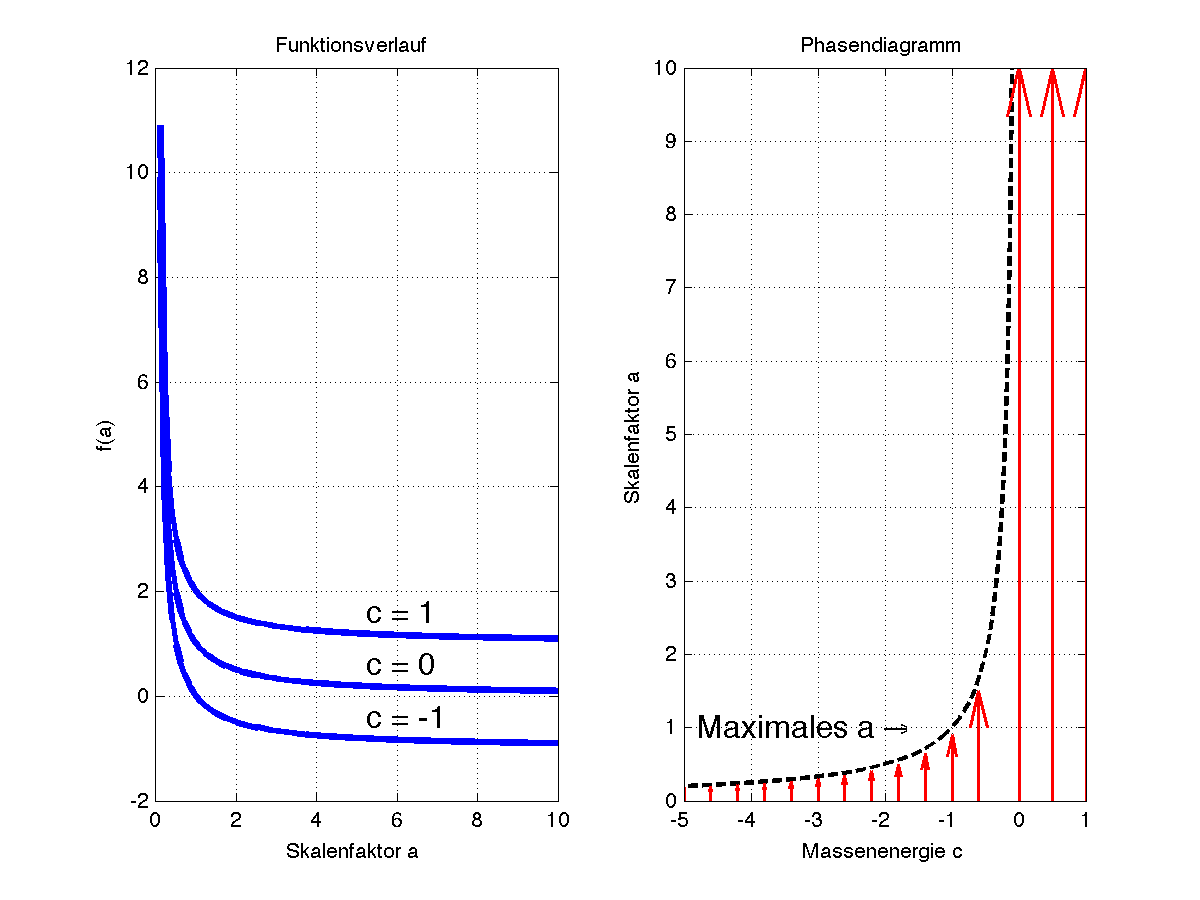
\includegraphics[width  = \textwidth]{friedmann/images/phasendiagramm.png}
	\caption{Phasenportrait in Abhängigkeit der Gesamtenergie c
		\label{friedmann:phasenportrait}}
\end{figure}%

%In \ref{friedmann:friedmannGleichung} sind die Differentialgleichungen in Abhängigkeit von c in MatLab numerisch aufgelöst werden. 
%
%\begin{figure}[h]
%	\centering
%	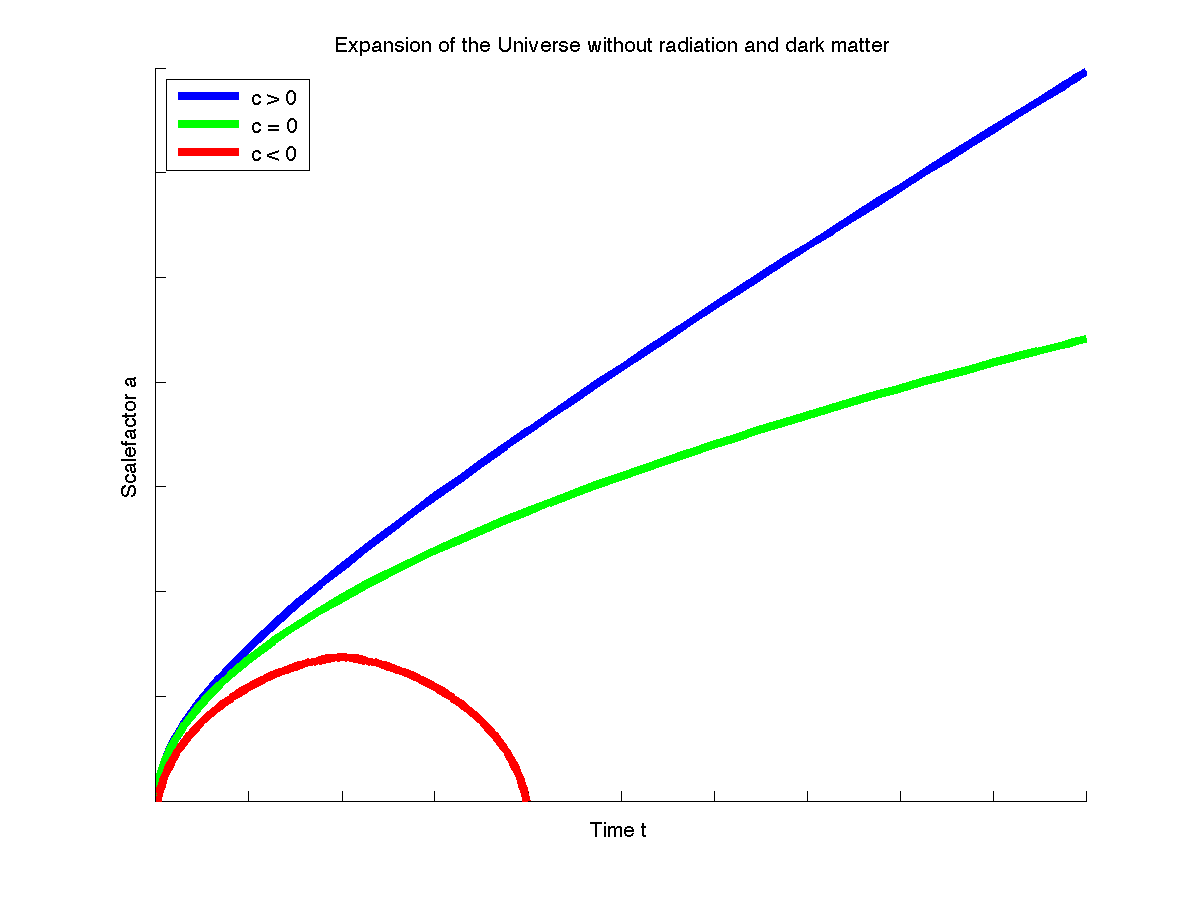
\includegraphics[width =  \textwidth]{friedmann/images/friedmann_ordinary_matter.png}
%	\caption{Verhalten des Universums in Abhängigkeit von der Zeit $t$
%		\label{friedmann:friedmannGleichung}}
%\end{figure}%
	

\subsection*{Energiedichte}
Wie wir wissen, existiert im Weltall nicht nur sichtbare, sondern auch dunkle Materie und Strahlung. Dunkle Materie verhält sich in Bezug auf die gravitative Wirkung ähnlich wie sichtbare Materie, und deshalb wird im Folgenden nicht weiter darauf eingegangen.
Anders verhält es sich mit der kosmischen Strahlung in Bezug auf die Dynamik des Kosmos. Wir schreiben


\[ E_{str} = \frac{h c}{\lambda} \]

wobei $h$ die \textbf{Planksche Konstante}, $c$ die \textbf{Lichtgeschwindigkeit} und $\lambda$ die \textbf{Wellenlänge} des Photons ist.
Nun ist die Energie der Strahlung (z.B. eines Photons) in einem sich ausdehnenden Universum nicht konstant, sondern ändert sich mit der Zeit. 
Denn, vergrössert sich die Raumzeit während der Laufzeit um einen Faktor n, so geschieht dies auch mit der Wellenlänge des Strahls.
Das bedeutet, dass die Energie eines Photons umgekehrt proportional zum Skalenfaktor a ist. Für die Energiedichte der Strahlung bedeutet dies, dass sie sich nicht nur kubisch wie bei der baryonischen Materie ändert, sondern mit vierter Potenz.
\begin{equation}
\rho_{str} = \frac{\nu}{a^4}
\end{equation}
In die Gleichung der Energieerhaltung des Universums setzen wir $\rho_{str}$ ein.
\[
\left(\frac{\dot{a}}{a} \right)^2 = \frac{8 \pi G}{3} \frac{\nu}{a^4} + \frac{c_2}{a^2 R^2}
\]
Vereinfacht
\[
\left(\frac{\dot{a}}{a} \right)^2 = \frac{1}{a^4} + \frac{c}{a^2} \Leftrightarrow \dot{a} = \sqrt{\frac{1}{a^2} + c}
\]

Wiederum ist die Differentialgleichung nicht elementar lösbar. Trotzdem können wir sagen, dass für \textbf{kleine} \textit{a's} der \textbf{erste} Term dominiert, während der \textbf{zweite} Term für \textbf{grosse} \textit{a's} dominiert.


Setzen wir die Gesamtenergie des Universums $c$ gleich null, findet sich die neue Gleichung	\[\left(\frac{\dot{a}}{a} \right)^2 = \frac{1}{a^4}\]
Um die Gleichung zu lösen, ziehen wir die Quadratwurzel und multiplizieren mit $a$.
\[ \dot{a} = \frac{1}{a} \]
\[\frac{da}{dt} =\frac{1}{a} \Leftrightarrow \frac{dt}{da} = a \]
\[ t = \frac{1}{2} a^{2} \Rightarrow a = \sqrt{2} \quad t^{1/2} \]

Analog zum Newtonschen Ansatz verhält sich das Universum für einen dominierenden zweiten Term gemäss Gleichung \ref{friedmann:LoesungZweiterTerm}.

\subsection{Relativistischer Ansatz}
Die bisher gemachten Überlegungen berücksichtigen nur die klassische oder newtonsche Physik, tatsächlich spielen die relativistischen Gesetze Einsteins eine wesentliche Rolle bei der Beschreibung des Kosmos.
Im vorhergehenden Abschnitt haben wir die Bedeutung der Massendichte "gewöhnlicher", sogenannter baryonischer Masse kennengelernt. Im relativistischen Ansatz geht es nun darum, die Geometrie des Raumes mit den Energiedichten in einen Zusammenhang zu bringen.
Die bereits hergeleitete Formel können wir so umschreiben, dass die linke Seite etwas mit der Geometrie des Raumes zu tun hat, während die rechte Seite die Energiedichte repräsentiert.
\begin{equation}
\left(\frac{\dot{a}}{a} \right)^2 - \frac{c}{a^2} = \frac{8 \pi G}{3} \rho 
\label{friedmann:Einstein}
\end{equation}



\subsection*{Geometrie des Raumes}
Wie wir zu beginn des Abschnitts erwähnt haben, muss die  linke Seite der Gleichung \ref{friedmann:Einstein} etwas mit der Geometrie des Raumes zu tun haben.
Der erste Term ist die Hubble-Konstante und beschreibt die Ausdehnung des Raumes. Das heisst
$c$ muss die Krümmung des Raumes wiedergeben.
Wir benennen die Konstante um zu
$-\kappa$ und schreiben die Gleichung neu:


\[ \left(\frac{\dot{a}}{a} \right)^2 + \frac{\kappa}{a^2} = \frac{8 \pi G}{3} \rho  \]

\begin{equation}
\left(\frac{\dot{a}}{a} \right)^2  = \frac{8 \pi G}{3} \rho  - \frac{\kappa}{a^2}
\end{equation}
\begin{table}[h]
\centering
\begin{tabular}{|>{$}r<{$}|>{$}r<{$}|>{$}c<{$}|}
\hline
\kappa&Geometrie&Winkelsumme\: \Delta\\
\hline
+1 & \text{Elliptisch} & > 180^\circ\\
0  & \text{Euklidisch} & =180^\circ\\
-1 & \text{Hyperbolisch} & <180^\circ\\
\hline	
\end{tabular}
\caption{Bedeutung von $\kappa$ für die Geometrie des Raumes}
\end{table} \linebreak
Die Krümmung des Raumes kann durch Messen von Winkelsummen im Dreieck bestimmt werden.

\subsection{kosmologische Rotverschiebung z}
Es stellt sich nun die Frage, wie sich die momentane Ausbreitungsgeschwindigkeit, also die Hubble-Konstante, feststellen lässt. Dabei nutzt man die Eigenschaft der Strahlung, dass sich die Wellenlänge proportional mit dem Raum mitdehnt. Diese Verschiebung der Wellenlänge in den roten Spektralbereich nennt man in der Kosmologie die \textit{kosmologische Rotverschiebung z}. Sie ersetzt oft die Angabe von Entfernungen, weil z einfacher zu bestimmen ist, als die tatsächliche Entfernung des kosmologischen Objekts. 
Kennt man nun die exakte Entfernung zu einem Objekt, kann zusammen mit dem \textit{Hubble-Gesetz} die Hubble-Konstante $H_0$ berechnet werden. Die Linearität des Hubble-Gesetz gilt jedoch nur bis zu einer Rotverschiebung von $z \sim 0.1$.

\[ cz = H_0 \, D \qquad \qquad \textbf{(Hubble-Gesetz)} \]
\[c = \text{Lichtgeschw. ; } H_0 = \text{Hubble-Konstante ; } D = \text{Distanz} \]
Der momentane Wert der Hubble-Konstante, den man in verschiedenen Literaturen nachschlagen kann, ist:
\[ H_0 = H(t_0) \approx (74.3 \pm 2.1) \frac{km}{s}\frac{1}{Mpc}\]

\end{refsection}
